\documentclass[tikz,border=0pt]{standalone}
\usepackage{tikz}
\usepackage{xcolor}

% Official HCMUT colors
\definecolor{hcmutblue}{RGB}{0,51,102}    % Official HCMUT blue
\definecolor{hcmutorange}{RGB}{255,102,0} % Official HCMUT orange

\begin{document}
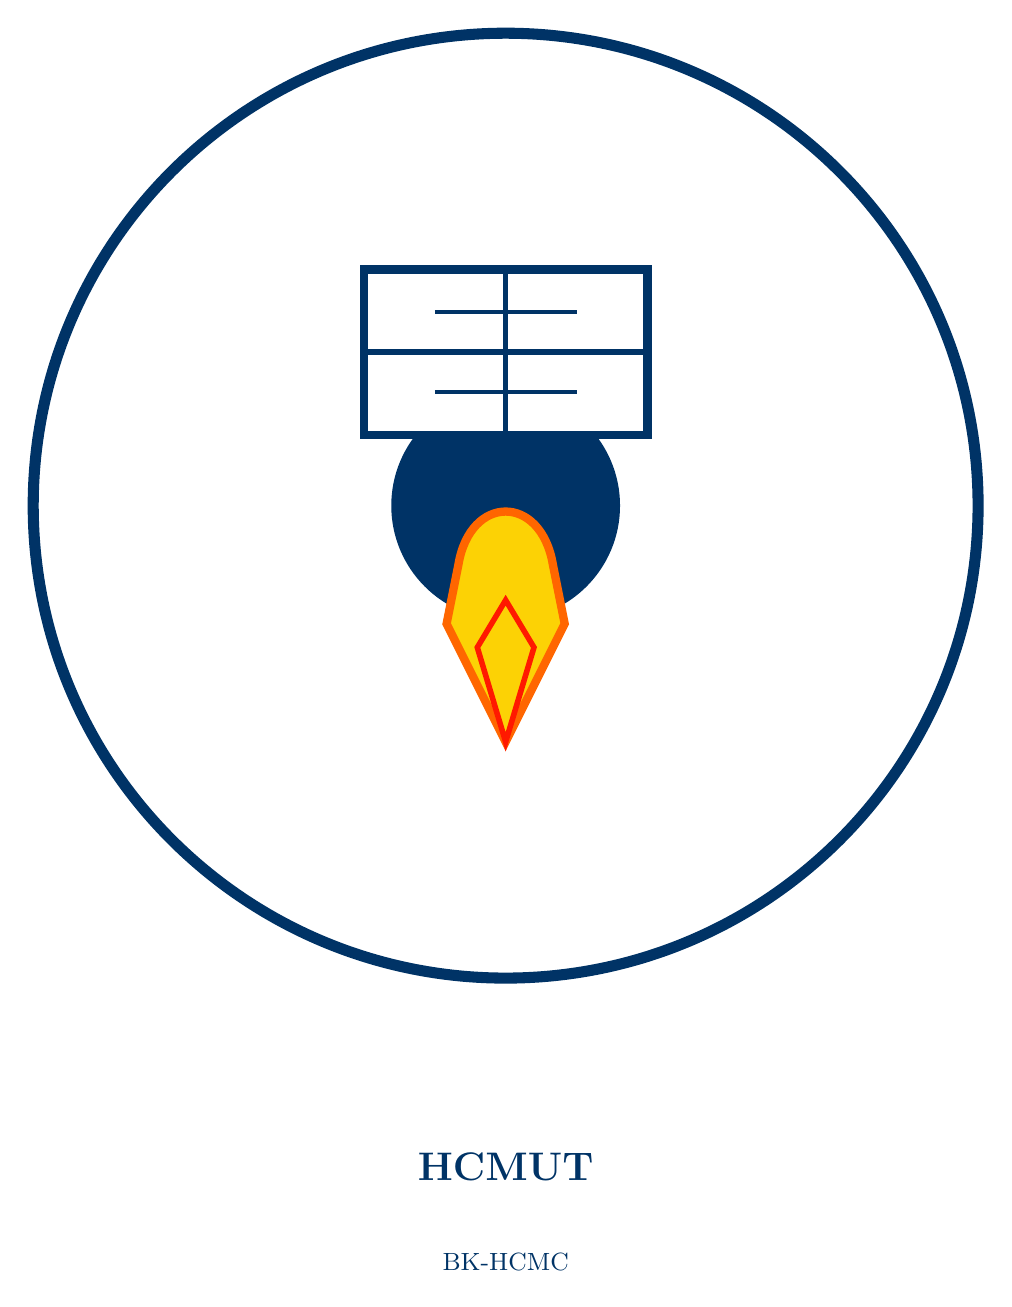
\begin{tikzpicture}[scale=3]
    % Outer circle with official HCMUT colors
    \draw[line width=4pt, color=hcmutblue] (0,0) circle (2cm);
    
    % Inner circle
    \node[circle, draw, fill=hcmutblue!10, minimum size=2.8cm, line width=3pt, color=hcmutblue] at (0,0) {};
    
    % Book symbol (detailed and professional)
    \draw[line width=3pt, color=hcmutblue, fill=white] (-0.6,0.3) rectangle (0.6,1.0);
    \draw[line width=2pt, color=hcmutblue] (-0.6,0.65) -- (0.6,0.65);
    \draw[line width=2pt, color=hcmutblue] (0,0.3) -- (0,1.0);
    \draw[line width=1.5pt, color=hcmutblue] (-0.3,0.48) -- (0.3,0.48);
    \draw[line width=1.5pt, color=hcmutblue] (-0.3,0.82) -- (0.3,0.82);
    
    % Torch/flame (realistic and professional)
    \draw[line width=3pt, color=hcmutorange, fill=yellow!70!orange] 
        (0,-1.0) -- (-0.25,-0.5) -- (-0.2,-0.25) 
        .. controls (-0.15,0.05) and (0.15,0.05) .. 
        (0.2,-0.25) -- (0.25,-0.5) -- cycle;
    
    % Flame details
    \draw[line width=2pt, color=red!80!orange] 
        (0,-1.0) -- (-0.12,-0.6) -- (0,-0.4) -- (0.12,-0.6) -- cycle;
    
    % Official text with proper typography
    \node[font=\Large\bfseries, color=hcmutblue] at (0,-2.8) {HCMUT};
    \node[font=\small, color=hcmutblue] at (0,-3.2) {BK-HCMC};
\end{tikzpicture}
\end{document}
